\chapter{Implementation}
In this chapter, we describe POXVine's implementation in detail. 

\section{MinSwitchMapper}
The POXVine System can use any host mapper heuristic to map the virtual hosts. For \emph{modularization}, each host mapper takes input the physical Topology and virtual Topology object and stores the mapping in text files for other modules of the system to use. This also allows us to use different host mappers simultaneously for different tenants. \\

MinSwitchMapper minimises the diameter of the network graph connecting the hosts of the virtual topology as seen in Chapter 5. Algorithm 1 is used to find the virtual-to-physical mapping which minimises the diameter. The intuition behind the algorithm is that the switches connected to hosts initially carry the capacity of the host. Every round, we \emph{percolate} the capacity to its neighbours, so, the first round we get a switch with capacity exceeding the required capacity, we can terminate the algorithm. A host list obtained in a \emph{later round} will have greater distance among hosts as we percolate to farther hosts each round, increasing the distance, and thus the diameter of the network graph formed by the virtual hosts. \\

Once the algorithm provides a list of physical hosts with sufficient capacity, we try to map the largest virtual host on the largest physical host, and if we can, repeat the step again till all the virtual hosts are mapped. If such a mapping is not possible, then we reiterate Algorithm 1 to find a different host list to map the virtual hosts. 

\IncMargin{1em}
\begin{algorithm}
  \SetKwData{swl}{swlist1}\SetKwData{round}{round}\SetKwData{Up}{up}
  \SetKwData{swll}{swlist2}
  \SetKwFunction{len}{len}\SetKwFunction{append}{append}
  \SetKwFunction{capacity}{capacity}\SetKwFunction{mapHosts}{mapHosts}
  \SetKwFunction{neighbours}{neighbours}
  \SetKwInOut{Input}{input}\SetKwInOut{Output}{output}
  \Input{Physical Topology $P$, Virtual Host List $vhosts$}
  \Output{Virtual-to-physical mappings of each host in $vhost$}
  \emph{Heuristic: Minimise the constructed network graph.}
  \BlankLine
  \emph{Initialization:}\\
  	\swl $\leftarrow$  [] \\
  	\swll $\leftarrow$ [] \\
  	\round $\leftarrow$ 0 \\
  \For{host in P.phosts}{
  	host$\rightarrow$switch$\rightarrow$hostlist = [host] \\
  	\swl.\append(host$\rightarrow$switch) \\
}
	\emph{Start the Percolation Rounds.}\\
  \While{MappingNotFound} {
  		\While{ \len(\swl) $\neq$ 0} {
  				sw = \swl.pop() \\
  				\If{ \capacity( sw$\rightarrow$hostlist ) $\ge$ \capacity(vhosts)} {
  					MappingNotFound = False \\
  					\mapHosts ( sw$\rightarrow$hostlist )
  				}
  				nlist = \neighbours(sw) \\
  				\For{n in nlist} {
  					\emph{Add all the hosts in sw$\rightarrow$hostlist to n$\rightarrow$hostlist} without duplicates.\\ 
  					If any change in n$\rightarrow$hostlist, add n to \swll
  				}			
  		}
  		\swl $\leftarrow$ \swll \\
  		\swll $\leftarrow$ [] \\
  		\round $\leftarrow$ \round + 1
	}
  \caption{Minimum Network Diameter Host Mapping Algorithm}\label{algo_disjdecomp}
\end{algorithm}\DecMargin{1em}

\section{NetworkMapping}
The NetworkMapping class uses the \emph{virtual-to-physical} mappings provided by the host mapper, and calculates all the network routes on the physical topology required for the virtual hosts to talk to each other. Consider the topology in Figure 4.3. The NetworkMapping object will first find the route from $v1$ to $v2$ in the virtual topology, that is $v1 \rightarrow vs1 \rightarrow vs2 \rightarrow v2$.  \\

The Physical Topology object has a method \verb|getCompleteRoute()| which translates the virtual route to the corresponding physical topology route by finding the physical route for each hop in the virtual topology. Thus, from the virtual route, we obtain the following physical route : $v1 \rightarrow s1 \rightarrow s2 \rightarrow s3  \rightarrow vs1 \rightarrow s3 \rightarrow s2  \rightarrow s1 \rightarrow vs2 \rightarrow s1  \rightarrow s2 \rightarrow s3 \rightarrow v2$. \\
\begin{center}
	Pseudo Code for Network Route Generation
\end{center}
\begin{lstlisting}
for each pair of virtual hosts{h1, h2}) : 
  virtualRoute = virtualTopology.getRoute(h1, h2)
  physicalRoute = 
    physicalTopology.getCompleteRoute(virtualRoute)
  physicalRoute.setRouteTags()
  add physicalRoute to networkPaths
end for
\end{lstlisting}
Note that we need to add rules from $v1$ to $v2$ and the other way as well, $v2$ to $v1$. After generating all the routes for a virtual topology, this is passed to the NetworkMapper module, which translates them into OpenFlow rules to install at the respective switches. 

\section{NetworkMapper}
\subsection{Route Tagging}
\begin{figure}
	\noindent
	\makebox[\textwidth]{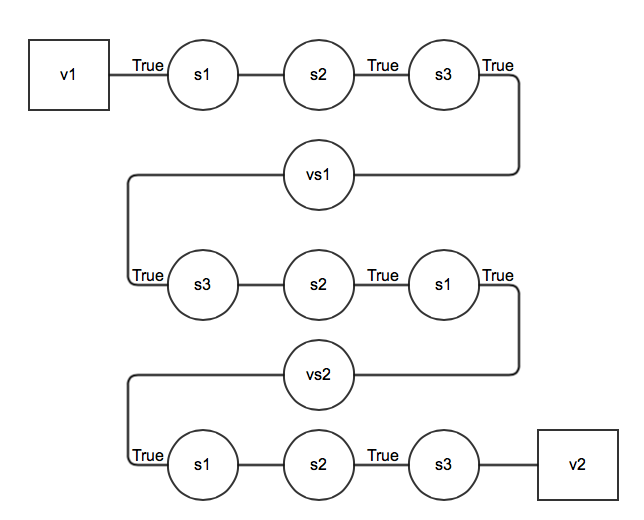
\includegraphics[width=17cm]{Figures/routetag.png}}%
	\caption{Setting Up Route Tags}
\end{figure}
The NetworkMapper is a POX application. Using the NetworkMapping object, it obtains all the routes it needs to install OpenFlow rules for at the mininet switches. As discussed in the previous chapter, we need \emph{Route Tags} to distinguish between different segments in the network route. The Route class has a function \verb|SetRouteTags()| which differentiates the segments and marks those switches in the route where there is a need to match and increment the route tags (start and end of segments). We illustrate an example in Figure 5.1. \\
The technique of finding these route tags is, in a network, the start and end of a segment will always be a \emph{virtual entity}. Thus, the switch preceeding and succeeding the virtual entity(will be the same in our case) will need to check and increment the Route Tag. This is done by the function \verb|SetRouteTags()|. 

\subsection{Proactive Rule Installation}
When a packet reaches a switch which does not have any rule for the packet, a \emph{PacketIn} message is sent to the POX Controller which can install the rule for the corresponding packet at the switch. However, this \emph{reactive} rule installation will have increased latencies for the first flows. POXVine, after receiving the first packet, \emph{proactively} installs all the network rules across all the switches (which will take some time), but any new flow will not be suffer from increased latency due to addition of OpenFlow rules by the controller. However, one problem with \emph{proactive} rule installation is that we need to add rules for communication for all hosts to all other hosts for all tenants, which can impose resource constraints on the switch flow table sizes, thus hindering scalability. With \emph{reactive} rule installation, you add only rules for hosts which are communicating with one other. 

\subsection{Discovery}
The POX distribution comes with many useful applications. One of them is \emph{Discovery} module, which helps detect the links in the topology. Using this, the NetworkMapper can create the \emph{port map} for each switch(the mapping of switch port and neighbour). This is then used by to install the required rules (therefore, POXVine should not start the installation of rules before all the link discoveries have been received by the controller.) Another use of the Discovery module is that in case of link failures, the NetworkMapper must set up alternate routes to maintain connectivity. 

\subsection{Notes}
\begin{itemize}
	\item ARP packets are tricky to handle (in general, broadcast is in such a system). The virtual hosts do not need a ARP protocol for communication, however, to adhere to legacy protocols, ARP packets are flooded across the network. 
	\item To check IP headers at the switch, we need the packet to match this.
	\begin{center}
						\verb|msg.match.dl_type = ethernet.IP_TYPE|
	\end{center}
	\item The \emph{VLAN ID} header field is used to store the tenant ID and RouteTag. The 12=bit VLAN ID has tenant ID as the most significant 6 bits and route tag as the least significant 6 bits.
	\item To send a packet back the input port (in case of loops), the controller needs to add a pecial rule and the outport should be \emph{OFFP\_IN\_PORT}.
\end{itemize}

